\documentclass{article}
\usepackage{amsmath}
\usepackage{tikz}

\title{Quantile Plots: Penguin Body Masses}
\author{}
\date{}

\begin{document}

\maketitle

\section*{Introduction}

We have used the \textbf{median}, the value with 50\% of observations to its left, to measure the centre of a distribution. Additionally, we use the \textbf{first quartile}, with 25\% of observations to its left, and the \textbf{third quartile}, with 75\% to its left, to measure spread. These percentiles are used to construct a \textbf{box plot}, which provides insight into the shape of a distribution.

\section*{Quantiles}

Beyond these percentiles, we can define other quantiles, such as the 10th percentile, which has 10\% of the observations to its left. A quantile is essentially a percentile expressed as a proportion. For example, the median is the 0.5 quantile, and the first quartile is the 0.25 quantile.

A \textbf{quantile plot} shows the observations for a variable, plotted against their corresponding quantile. Below is a simple representation of a quantile plot using LaTeX and TikZ, which demonstrates how body mass data might be represented in such a plot.

\begin{center}
\begin{tikzpicture}
    \draw[->] (0,0) -- (10,0) node[right] {Quantiles};
    \draw[->] (0,0) -- (0,6) node[above] {Body Mass (g)};
    
    % Draw quantiles
    \draw (1,1) -- (1,1) node[below] {0.1};
    \draw (2,2) -- (2,2) node[below] {0.2};
    \draw (3,3) -- (3,3) node[below] {0.3};
    \draw (4,4) -- (4,4) node[below] {0.4};
    \draw (5,4.5) -- (5,4.5) node[below] {0.5 (Median)};
    \draw (6,5) -- (6,5) node[below] {0.6};
    \draw (7,5.2) -- (7,5.2) node[below] {0.7};
    \draw (8,5.4) -- (8,5.4) node[below] {0.8};
    \draw (9,5.5) -- (9,5.5) node[below] {0.9};
    
    % Dotted lines for median and quartiles
    \draw[dotted] (0,4.5) -- (5,4.5) node[left] {4000g};
    \draw[dotted] (0,3) -- (3,3) node[left] {3000g};
    \draw[dotted] (0,5.5) -- (9,5.5) node[left] {5000g};
\end{tikzpicture}
\end{center}

In this plot, the median body mass is approximately 4000 g, and the interquartile range (IQR) is around 1200 g (between the 25th and 75th percentiles).

\section*{Comparing Distributions}

Quantile plots are particularly useful for comparing distributions. Below is an example of a basic quantile plot comparing three penguin species: \textbf{Adélie}, \textbf{Chinstrap}, and \textbf{Gentoo}.

\begin{center}
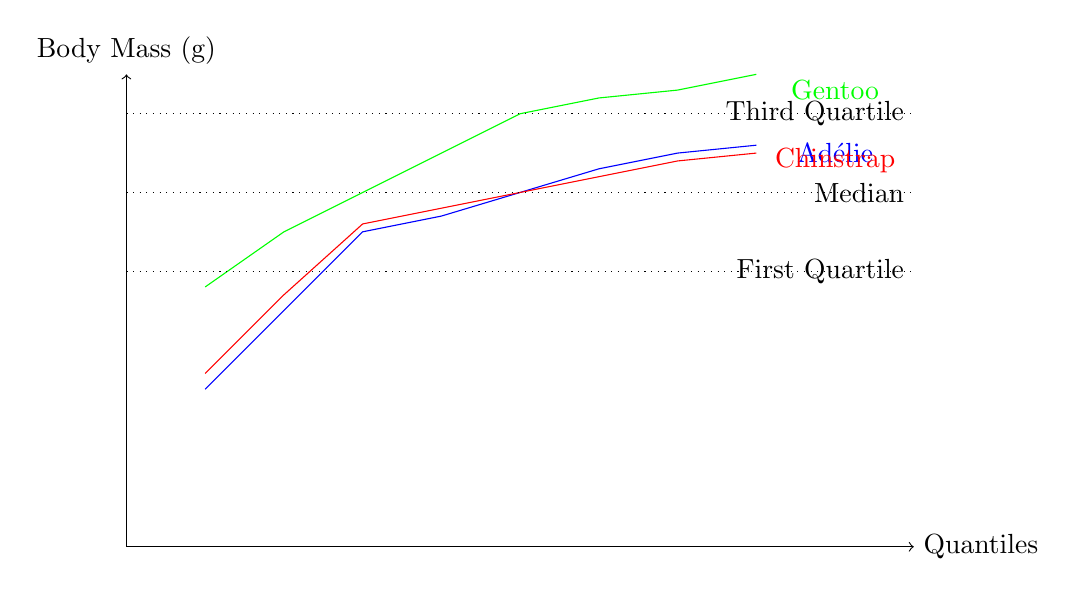
\begin{tikzpicture}
    \draw[->] (0,0) -- (10,0) node[right] {Quantiles};
    \draw[->] (0,0) -- (0,6) node[above] {Body Mass (g)};
    
    % Adélie
    \draw[blue] (1,2) -- (2,3) -- (3,4) -- (4,4.2) -- (5,4.5) -- (6,4.8) -- (7,5) -- (8,5.1);
    \node[blue] at (9,5) {Adélie};

    % Chinstrap
    \draw[red] (1,2.2) -- (2,3.2) -- (3,4.1) -- (4,4.3) -- (5,4.5) -- (6,4.7) -- (7,4.9) -- (8,5);
    \node[red] at (9,4.9) {Chinstrap};

    % Gentoo
    \draw[green] (1,3.3) -- (2,4) -- (3,4.5) -- (4,5.0) -- (5,5.5) -- (6,5.7) -- (7,5.8) -- (8,6);
    \node[green] at (9,5.8) {Gentoo};
    
    % Median lines
    \draw[dotted] (0,4.5) -- (10,4.5) node[left] {Median};
    \draw[dotted] (0,3.5) -- (10,3.5) node[left] {First Quartile};
    \draw[dotted] (0,5.5) -- (10,5.5) node[left] {Third Quartile};
\end{tikzpicture}
\end{center}

In this plot, we see that the distribution for Gentoo penguins is shifted upwards by about 1300 g compared to Adélie and Chinstrap penguins.

\section*{Multiple Choice}

The plot suggests that the body mass distributions of Adélie and Chinstrap penguins have a similar location (both have a median of 3700 g). However, the plot suggests that:

\begin{itemize}
    \item The variability in Adélie body mass is greater than the variability in Chinstrap body mass.
    \item \textbf{The variability in Chinstrap body mass is greater than the variability in Adélie body mass. (correct)}
    \item The variability in body mass is the same for Adélie and Chinstrap penguins.
\end{itemize}

\end{document}
